\subsection{The ALICE Detector}
\begin{itemize}
    \item What is the LHC?
    \item What is ALICE?
    \item What does ALICE look for?
    \item What is Run 3?
\end{itemize}
The ALICE detector (A Large Ion Collider Experiment) is a detector experiment at the Large Hadron Collider (LHC) at CERN. Its primary goal is the investigation of ``strongly interacting matter at extreme energy densities, where a formation of a new phase of matter, the quark-gluon plasma, is expected'' \cite{ALICE_LOI}. It achieves this goal by studying the products of head-on collisions of heavy ions such as lead. 

% ALICE is situated at 

% The LHC at CERN in Geneva is built to accelerate particles up to very high energies (\SI{13.6}{\tera\electronvolt})

The coordinate system used at ALICE needs to be discussed first in order to fully explain the scope of this report. A modified cylindrical coordinate system, shown in \cref{fig:coords} \cite{coords}, is used as most detectors in the experiment are cylindrically symmetric about the beamline of the LHC. 

\begin{figure}[h]
    \begin{center}
        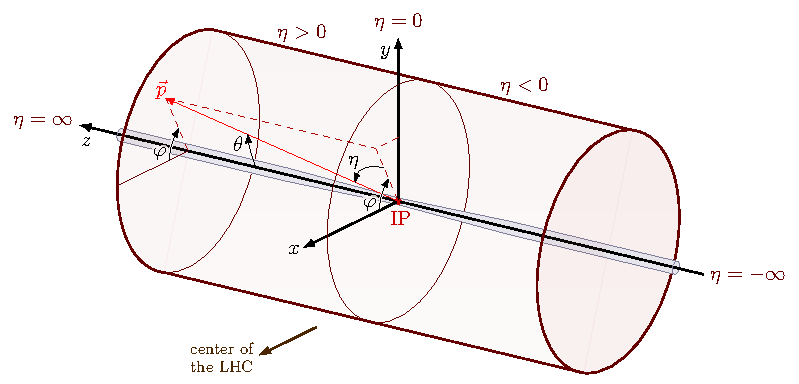
\includegraphics[width=.8\textwidth]{Figs/coords.pdf}
        \caption{Modified cylindrical coordinate system used at the LHC \cite{coords}}
        \label{fig:coords}
    \end{center}
\end{figure}

We place the $z$-axis along the beamline with its origin at the interaction point (IP). The IP is the point at which collisions happen, right in the center of the detector. The angle around the $z$-axis is $\varphi$; the azimuthal angle. The angle from the $z$-axis to the $x-y$ plane is called $\theta$; the polar angle. We are interested in the momentum of particles that we track in the detector, which we call $\vec{p}$, but we also define the transverse momentum as 
\begin{equation}
    p_{\mathrm{T}}=\sqrt{p_x^2 + p_y^2}.
    \label{eqn:transverse momentum}
\end{equation}
We define the rapidity, often denoted as $y$, as
\begin{equation}
    y=\frac 12 \ln\left(\frac{E+p_z}{E-p_z}\right)
    \label{eqn:rapidity}
\end{equation}
where $E$ is the total energy of the particle being considered and $p_z$ is the momentum in the $z$ direction \cite{kar_exp_phys}. This quantity is useful as differences in rapidity aer Lorentz invariant for boosts along the $z$-axis. One issue, however, is that the energy $E$ is hard to measure, so we instead use pseudorapidity, denoted as $\eta$. Rapidity and pseudorapidity are equivalent for massless particles, and near equivalent for particles with high energies such that their total 3-momentum magnitude $p$ is much greater than their mass $m$. Pseudorapidity is much easier to measure as it is defined as \cite{kar_exp_phys}
\begin{equation}
    \eta=-\ln\tan\frac{\theta}{2}.
    \label{eqn:pseudorapidity}
\end{equation}
From \cref{fig:coords} we see that for $z$ positive, $\eta$ is also positive, and similarly for $z$ negative. Confusingly, we define the ``forward region'' of the ALICE detector as the region for which $z$, and thus $\eta$, are negative. 

The LHC Long Shutdown 2 (LS2), which started in 2018, is followed by what is called Run 3. Significant upgrades were made to ALICE during LS2 for Run 3. \Cref{fig:ALICE_Schematic} shows the detector configuration for Run 3. The intent of these upgrades was in large part to prepare ALICE for higher frequency collisions in both Pb-Pb and p-p cases. 

\begin{figure}[h]
    \begin{center}
        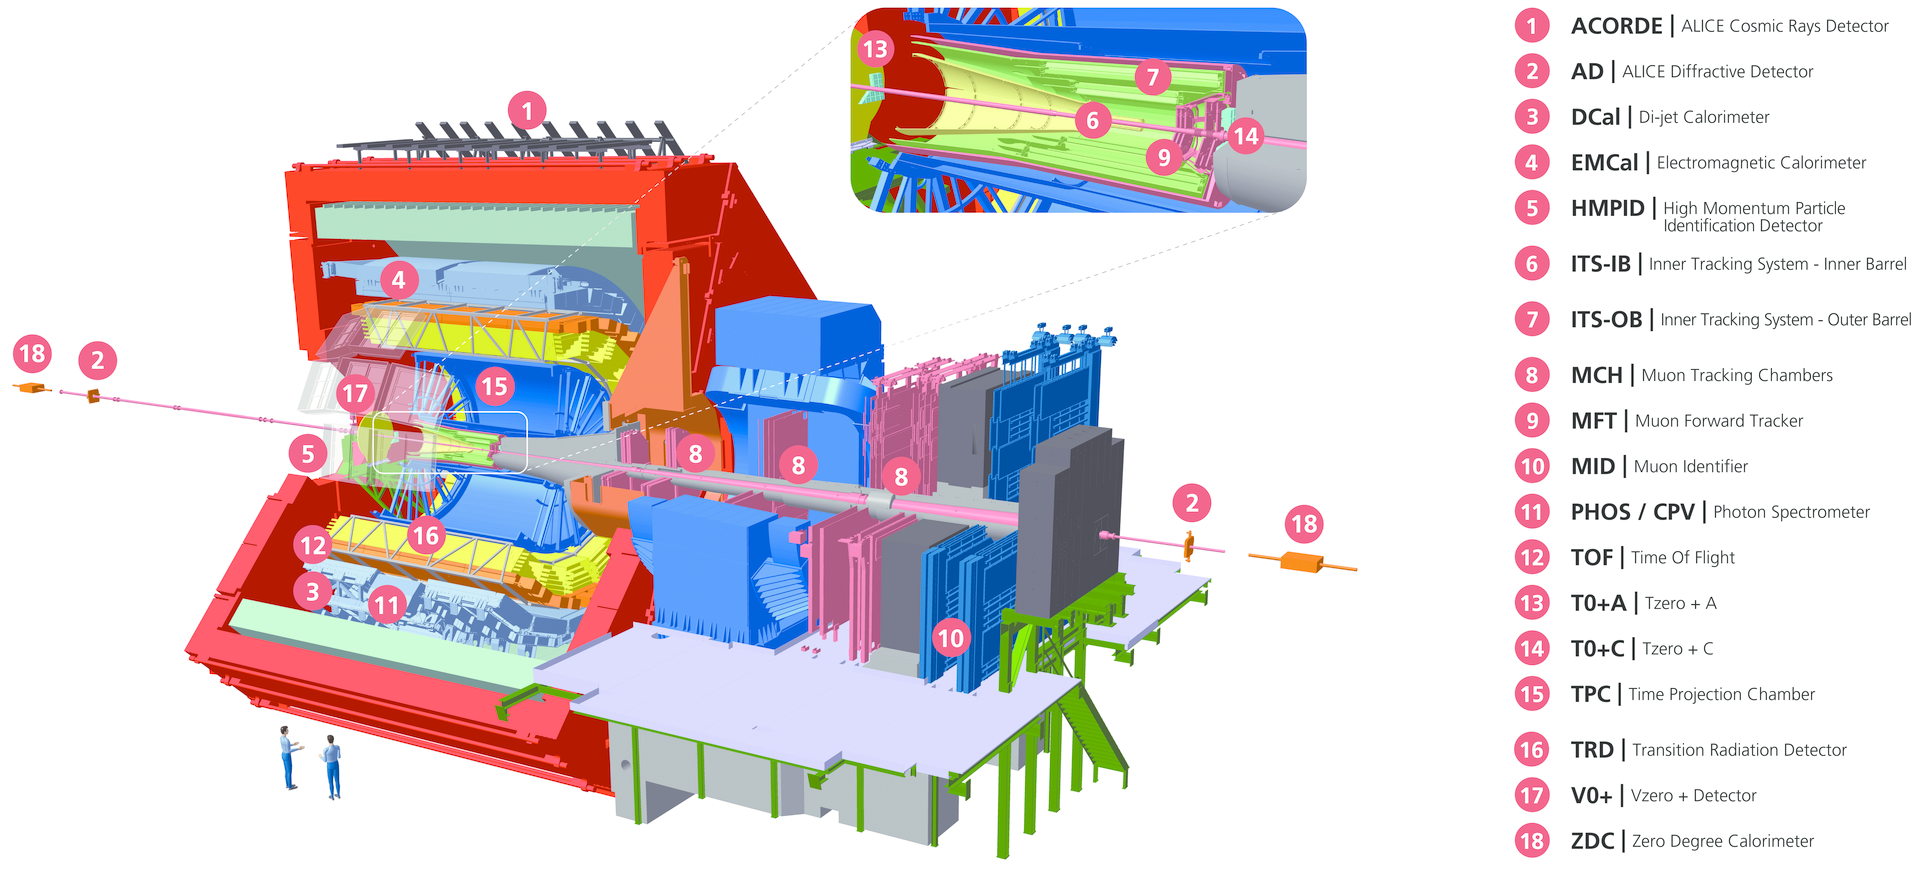
\includegraphics[width=.8\textwidth]{Figs/ALICE_RUN3_schematic.png}
        \caption{ALICE Run 3 schematic}
        \label{fig:ALICE_Schematic}
    \end{center}
\end{figure}

Part of the upgrades for Run 3, the details of which can be found in \cite{ALICE_Upgrade_LOI}, were a whole new Inner Tracking System (ITS) and a brand new detector called the Muon Forward Tracker (MFT). These detectors are both silicon-based, and as can be deduced from their names are made for tracking particles. 


\subsection{Muon Forward Tracker}